\documentclass[tikz,border=12pt]{standalone}
\usepackage{fontspec}
\setmainfont{Segoe UI}
\usepackage{amsmath,amssymb}
\usepackage{tikz}

\usetikzlibrary{calc,arrows.meta}

\begin{document}
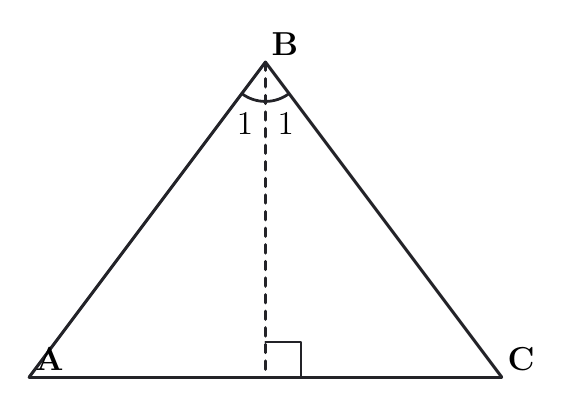
\begin{tikzpicture}[x=1.0000cm,y=1cm,line cap=round,line join=round]
\definecolor{linec0}{RGB}{35,35,40}
\definecolor{linec1}{RGB}{35,35,40}
\definecolor{linec2}{RGB}{35,35,40}
\definecolor{linec3}{RGB}{35,35,40}
\definecolor{linec4}{RGB}{35,35,40}
\definecolor{linec5}{RGB}{35,35,40}
\definecolor{edgecol}{RGB}{35,35,40}
\definecolor{hicol}{RGB}{35,35,40}
\definecolor{angcol}{RGB}{35,35,40}
\coordinate (A) at (-3.0000,0.0000);
\coordinate (H) at (0.0000,0.0000);
\coordinate (C) at (3.0000,0.0000);
\coordinate (B) at (0.0000,4.0000);
\draw[edgecol,line width=1.1pt] (A) -- (B);
\draw[edgecol,line width=1.1pt] (B) -- (C);
\draw[edgecol,line width=1.1pt] (C) -- (A);
\draw[edgecol,line width=1.1pt,dashed] (B) -- (H);
\draw[edgecol,line width=0.7pt] (0.000,0.450) -- (0.450,0.450) -- (0.450,0.000);
\draw[edgecol,line width=1.00pt] (0.000,4.000)++(-126.87:0.500) arc[start angle=-126.87, delta angle=36.87, radius=0.500];
\node[text=black,font=\large] at (-0.259,3.222) {1};
\draw[edgecol,line width=1.00pt] (0.000,4.000)++(-90.00:0.500) arc[start angle=-90.00, delta angle=36.87, radius=0.500];
\node[text=black,font=\large] at (0.259,3.222) {1};
\node[font=\bfseries\large,inner sep=2pt,anchor=south west] at (-3.000,0.000) {A};
\node[font=\bfseries\large,inner sep=2pt,anchor=south west] at (0.000,4.000) {B};
\node[font=\bfseries\large,inner sep=2pt,anchor=south west] at (3.000,0.000) {C};
\end{tikzpicture}
\end{document}
